\documentclass[10pt,twocolumn,letterpaper]{article}

\usepackage[utf8]{inputenc}
\usepackage[english]{babel}
\usepackage{graphicx}
\usepackage[colorlinks=true, allcolors=blue]{hyperref}
\usepackage[margin=0.7in, columnsep=0.28in]{geometry}
\usepackage{titlesec}
\usepackage{caption}
\usepackage{abstract}
\usepackage{amsmath}
\usepackage{amssymb}
\usepackage{booktabs}
\usepackage{microtype}
\usepackage{float}
\usepackage{url}

\raggedbottom
\tolerance=2000
\emergencystretch=15pt

\setlength{\textfloatsep}{10pt plus 1.0pt minus 2.0pt}
\setlength{\intextsep}{10pt plus 1.0pt minus 2.0pt}

\titleformat{\section}{\large\bfseries}{\thesection.}{0.5em}{}
\titleformat{\subsection}{\normalsize\bfseries}{\thesubsection.}{0.5em}{}
\titlespacing*{\section}{0pt}{11pt}{4pt}
\titlespacing*{\subsection}{0pt}{8pt}{3pt}

\captionsetup{font=small, labelfont=bf}

\title{\vspace{-2.0cm}\LARGE\textbf{Designing a Phase II Trial Around One Fragile Subgroup:
Enrichment, Multiplicity, and Probability of Success for a Cardiac Extracellular Matrix Hydrogel}}

\author{
    \large \textbf{Palash Rakshit} \\
    \normalsize Independent Researcher, Redlands, California \\
    \normalsize \href{mailto:palash.raks@gmail.com}{palash.raks@gmail.com} \\
    \normalsize Code and data: \href{https://github.com/palashraks-afk/ventrigel-cds}{github.com/palashraks-afk/ventrigel-cds}
}
\date{}

\begin{document}

\twocolumn[
  \begin{@twocolumnfalse}
    \maketitle
    \vspace{-1.1cm}
    \begin{center}\large\textbf{Abstract}\end{center}
    \noindent\normalsize
    \textbf{Background.} The VentriGel first-in-man trial (NCT02305602) treated 15 post-infarction
    patients with an injectable decellularized porcine myocardial matrix and reported, post hoc,
    that improvements in left ventricular remodeling appeared mainly in patients treated more than
    twelve months after infarction. Whether that observation can support a Phase II design has not
    been quantified.
    \textbf{Methods.} No simulated patients were used. The trial's Supplemental Appendix reports
    every endpoint as mean with standard error and $n$, separately for the early ($<$12 months) and
    late ($>$12 months) strata, which determines the standard deviation exactly through
    $\mathrm{SD}=\mathrm{SEM}\sqrt{n}$. Transcription was validated by recomputing all 38 checkable
    published paired $t$-test $p$-values and by reconstructing each pooled mean and variance from
    its strata. The between-stratum interaction, which the trial did not test, was then evaluated
    and corrected for multiplicity. The missing control arm was anchored to placebo arms of five
    published trials rather than assumed. Trial size was computed as a function of enrichment, and
    reported as assurance -- power integrated over the uncertainty in the effect -- rather than as
    nominal power.
    \textbf{Results.} All 38 $p$-values reproduced; median SD reconstruction error was 3.3\% (0.3\%
    for end-systolic volume). Exactly one of nine endpoints shows a nominally significant
    interaction (end-systolic volume, $-16.9$ mL, 95\% CI $-32.2$ to $-1.6$, $p=0.034$), and it
    survives neither Bonferroni nor Benjamini--Hochberg correction. The strata are balanced on all
    eight baseline measures and the pattern runs opposite to regression to the mean. External
    control arms show that post-infarction natural history is era-dependent and disagrees in sign
    for acute patients ($-14.8$ to $+8.2$ mL) while chronic populations are stable ($0.0$ mL). Under
    anchored controls an unselected Phase II requires 1{,}046 patients against 92 enriched, but the
    same design has only 68\% probability of success; genuine 80\% assurance requires 174 patients
    and 17--21 sites, and no sample size exceeds a 97.5\% ceiling.
    \textbf{Conclusions.} The Phase I supports a fragile, multiplicity-sensitive signal of effect
    modification, not an established one. Conditional on it being real, enrichment is the difference
    between a feasible trial and an infeasible one; the entire conclusion rests on a single
    unmeasured quantity, the six-month volume change in untreated chronic post-infarction patients,
    for which the two available published estimates disagree.
    \vspace{0.35cm}

    \begin{center}\large\textbf{Disclosures}\end{center}
    \noindent\small This is an independent secondary analysis of published summary statistics. It was
    not conducted with, funded by, or endorsed by Ventrix, Inc., the Christman Laboratory, or any
    trial investigator. No patient-level data were accessed. The author declares no competing
    interests.
    \vspace{0.5cm}
  \end{@twocolumnfalse}
]

\section{Introduction}

A Phase I trial that establishes safety leaves a sponsor with a design question rather than an
answer: how large must the next trial be? For cardiovascular regenerative therapies the question is
often decisive. Phase II costs scale steeply with enrollment~\cite{moore2018}, success rates from
Phase II onward are low~\cite{wong2019}, and single-asset sponsors frequently exhaust their capital
between the two phases.

Restricting enrollment to patients more likely to respond --- \emph{enrichment} --- is an
established regulatory strategy for exactly this situation~\cite{fda2019, temple2010}. What is less
often made explicit is that the gain from enrichment depends on the \emph{structure} of the
heterogeneity, not merely its presence, and can be negative.

The usual description is that broad criteria ``dilute'' an effect. Dilution presumes the added
patients contribute a smaller benefit, so a larger trial eventually succeeds. If instead they
contribute a benefit of the \emph{opposite} sign, the pooled estimate is driven toward zero and can
cross it, and no trial of any size succeeds. The two cases are indistinguishable in a summary table
--- both show a small pooled effect --- and they imply opposite decisions.

The VentriGel first-in-man trial supplies an unusually clean instance of the second
case~\cite{traverse2019}. Fifteen patients with prior ST-segment elevation myocardial infarction and
moderate left ventricular dysfunction received transendocardial injections of a hydrogel derived
from decellularized porcine myocardial extracellular matrix~\cite{singelyn2009, seifnaraghi2013}.
The trial was single-arm and not powered for efficacy; one stated purpose was to inform which
patients a later trial should enroll~\cite{traverse2019}.

This paper asks what that finding implies quantitatively, and --- equally --- how much of it
survives scrutiny. It does not attempt to predict whether an individual patient will respond, a
claim fifteen single-arm patients cannot support and which is separately problematic on statistical
grounds~\cite{senn2004}.

\subsection{Correction of a prior version}

An earlier version of this project, archived at
\href{https://doi.org/10.5281/zenodo.21516443}{10.5281/zenodo.21516443}, took the opposite approach:
it generated 2{,}000 synthetic patient records from a hand-written eligibility scoring rule, trained
a classifier to predict the resulting label, and reported a test ROC-AUC of 1.00.

That result was circular and the present paper supersedes it. The target variable was a
deterministic threshold function of the same features supplied to the classifier, so the model
recovered a conditional statement its author had written; the accuracy was an arithmetic consequence
of the construction. Reported feature importances reproduced hand-chosen penalty weights, and a
described hyperparameter search does not appear in the code. The classifier is retained in the
repository under \texttt{deprecated/} with a written account of the error. This correction is stated
prominently because the superseded version carries a DOI and may be encountered independently.

\section{Methods}

\subsection{Recovering the variance structure}

The Supplemental Appendix reports each endpoint as a mean with standard error and contributing $n$,
separately for the total cohort and the two temporal strata. Because
$\mathrm{SEM}=\mathrm{SD}/\sqrt{n}$,
\begin{equation}
\mathrm{SD} = \mathrm{SEM}\sqrt{n},
\end{equation}
which supplies everything a power calculation requires. No quantity in this study was digitized from
a figure, imputed, or simulated. Nine endpoints were transcribed with their source table recorded
alongside each value.

\subsection{Validating the transcription}

\textbf{Check 1.} The trial compared each visit against baseline with a paired $t$-test, so
$t=\text{mean}/\mathrm{SEM}$ on $n-1$ degrees of freedom. Recomputing every published $p$-value from
the transcribed statistics tests transcription, Equation~1, and the stated test simultaneously.

\textbf{Check 2.} The pooled cohort is the union of the strata, so its moments follow by the laws of
total expectation and total variance:
\begin{align}
\mu &= \textstyle\sum_g w_g\,\mu_g,\\
\sigma^2 &= \underbrace{\textstyle\sum_g w_g\,\sigma_g^2}_{\text{within}}
          + \underbrace{\textstyle\sum_g w_g\,(\mu_g-\mu)^2}_{\text{between}}.
\end{align}
Published totals were never inputs, so agreement is a genuine test, and a demanding one: the
between-stratum term is driven by exactly the separation the rest of the analysis depends on.

\subsection{Testing whether the subgroup effect exists}

The trial compared each stratum against its own baseline and observed that one reached significance
while the other did not. That is not a test of effect modification; two subgroups can fall on
opposite sides of $p=0.05$ without differing from each other, and this is among the most common
errors in subgroup reporting~\cite{wang2007, sun2010}. The between-stratum difference was therefore
tested directly with Welch's unequal-variance $t$-test on the change scores, using the recovered
standard deviations.

The trial states that it made no adjustment for multiple comparisons, which is appropriate for an
exploratory Phase I but means nominal $p$-values cannot be read as evidence strength here. Both
Bonferroni and Benjamini--Hochberg~\cite{benjamini1995} corrections were applied across the nine
interaction tests. A reduced denominator is also reported, since ejection fraction is algebraically
determined by the two volumes and viable mass and scar fraction partition the same myocardium; it is
presented alongside the nominal count rather than instead of it, because selecting the smaller
denominator after seeing the $p$-values would itself be a form of selection.

Two artifacts capable of manufacturing a spurious subgroup effect were checked. Baseline balance was
tested on every reported baseline, since the strata were not randomized against each other.
Regression to the mean was assessed by asking whether the stratum with the more extreme baseline
moved further from the mean, which regression cannot produce.

\subsection{Anchoring the missing control arm}

The Phase I was single-arm, so the early--late contrast confounds effect modification with
differential natural history. Rather than sweeping an arbitrary range, the control-arm change was
anchored to published control and placebo arms of randomized trials measuring left ventricular
volumes over approximately six months in comparable populations: TIME~\cite{traverse2012},
PRESERVATION-I~\cite{rao2016} and EMPRESS-MI~\cite{carberry2025} for acute patients, and
FOCUS-CCTRN~\cite{perin2012} and FOCUS-HF~\cite{perin2011} for chronic ones. Indexed volumes were
converted at a body surface area of 1.9\,m$^2$; the assumption is checkable, since it implies a
VentriGel baseline index of 78.2\,mL/m$^2$ against 65.0\,mL/m$^2$ in the chronic FOCUS-CCTRN
population.

\subsection{Sizing the trial as a function of enrichment}

Let $\pi$ be the late fraction of the \emph{eligible pool} and $e$ the late fraction of
\emph{enrolled} patients, so $e=\pi$ is unselected and $e=1$ fully enriched. For treatment-arm change
$d_g$ and control-arm change $c_g$ in stratum $g$, and a winner's-curse discount $\lambda$,
\begin{equation}
\Delta(e) = \lambda \textstyle\sum_g w_g(e)\,(d_g - c_g), \quad w_{\text{late}}(e)=e,
\end{equation}
with variance given by Equation~3 at $w_g(e)$. The discount multiplies the treatment-versus-control
difference rather than the raw change, since the winner's curse inflates the estimated \emph{effect}
of having selected the subgroup and says nothing about how much of the raw change was natural
history. Required $n$ scales as $\sigma^2/\Delta^2$, so enrichment acts on both terms: it raises
$|\Delta|$ by removing patients who dilute or oppose the effect, and lowers $\sigma$ by eliminating
between-stratum heterogeneity. Sample size was solved against the noncentral $t$ rather than the
normal approximation. All designs use $\alpha=0.05$ two-sided and 10\% dropout.

A design whose effect points away from benefit still returns a finite $n$, because $n$ depends on
$\Delta^2$. Such an $n$ is the size needed to detect a difference of that magnitude in either
direction, which is not a trial capable of showing the therapy works. Every design is flagged for
the sign of its effect, and cost optimization is restricted to designs favouring treatment.

\subsection{Probability of success rather than power}

Sizing for 80\% power at a point estimate and then calling the result an 80\% trial promotes an
assumption to a fact. Assurance~\cite{ohagan2005} integrates power over the uncertainty in the effect,
\begin{equation}
A(n) = \mathbb{E}_{\theta}\!\left[\,\mathrm{power}(n,\theta)\,\right],
\end{equation}
with the expectation over the sampling distribution of the stratum's true mean and variance,
$\mu\sim\bar{x}+(s/\sqrt{n_g})\,t_{n_g-1}$ and $\sigma^2\sim(n_g-1)s^2/\chi^2_{n_g-1}$. Assurance is
evaluated with common random numbers across sample sizes, so the curve is exactly monotone rather
than carrying Monte Carlo noise.

\subsection{Screening burden, cost, and uncertainty}

Enrichment is not free. Randomizing $N$ patients at level $e$ from a pool of composition $\pi$
requires screening
\begin{equation}
S = \max\!\left(\frac{eN}{\pi},\; \frac{(1-e)N}{1-\pi}\right),
\end{equation}
whichever stratum is exhausted first. A cost model separates per-screen from per-patient cost and
derives duration from screening throughput; unit costs are planning assumptions, and the paper's
primary claims are sample-size ratios, which do not depend on them.

Estimation uncertainty is propagated by a parametric bootstrap that re-solves the whole design on
each of 4{,}000 draws from the distributions above. Draws whose effect reverses sign are retained as
infeasible rather than discarded, since discarding them would bias intervals optimistically.
Simulation is used in this study only to propagate uncertainty already present in the published
estimates or to map assumptions; it is never used to create observations.

\section{Results}

\subsection{The transcription is faithful}

All 38 checkable published $p$-values were reproduced at the precision the source prints. Four cells
were excluded for documented reasons rather than counted as failures: three B-type natriuretic
peptide cells, whose table reports percent change while its $t$-test column tests absolute values,
and total-cohort scar fraction, where the printed $0.50\,(1.9)$ at $n=12$ implies $p=0.80$ rather
than the printed $p=0.58$ --- an unresolved source discrepancy, recorded and not corrected.

Reconstructing each pooled cohort from its strata gave a median standard-deviation error of 3.3\%.
For end-systolic volume the reconstruction returned $-0.36$ mL against a published $-0.35$ mL and a
standard deviation of 14.26 mL against 14.22 mL, an error of 0.3\%. Since the totals were never
inputs, this establishes that the recovered stratum variances are correct.

\subsection{One fragile interaction}

\begin{figure*}[t]
\centering
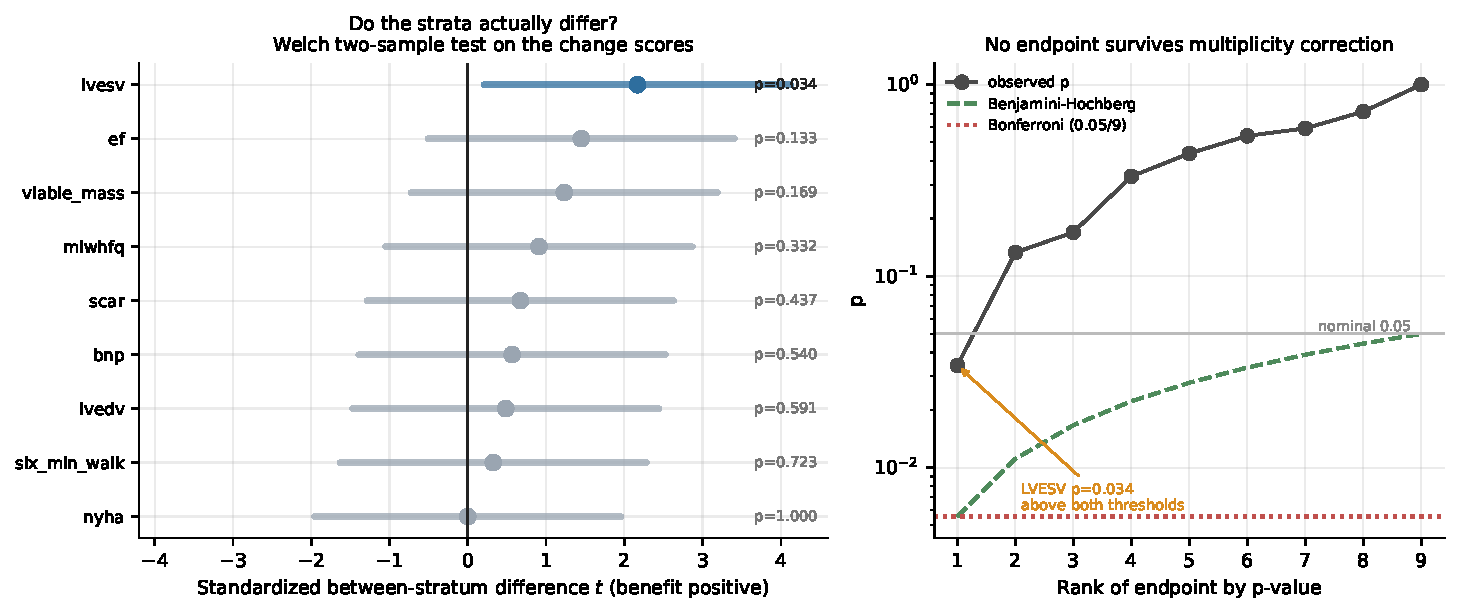
\includegraphics[width=\textwidth]{../results/figures/fig2_interaction_and_multiplicity.pdf}
\caption{Left: the between-stratum comparison the trial did not perform, standardized so endpoints
on different scales share an axis. Right: observed $p$-values against both multiplicity thresholds.
End-systolic volume is the only nominally significant interaction and it lies above both corrected
thresholds.}
\label{fig:interaction}
\end{figure*}

Figure~\ref{fig:interaction} gives the central inferential result. Exactly one of nine endpoints
shows a nominally significant interaction: end-systolic volume, with a between-stratum difference of
$-16.9$ mL (95\% CI $-32.2$ to $-1.6$, $p=0.034$). Ejection fraction ($p=0.13$), viable mass
($p=0.17$) and every remaining endpoint ($p>0.33$) do not.

It survives no correction. Bonferroni across nine tests requires $p<0.0056$; Benjamini--Hochberg at
$q=0.05$ rejects nothing. Collapsing the algebraically linked endpoints to five independent families
gives a threshold of $0.010$, which $p=0.034$ still fails.

Two checks come back in the finding's favour. The strata are balanced on all eight reported baseline
measures (minimum $p=0.46$; end-systolic volume 156.8 vs 142.3 mL, $p=0.68$), so the contrast is not
confounded by differing severity at entry. And the pattern runs opposite to regression to the mean:
the early stratum began with the \emph{higher} end-systolic volume and got worse, whereas regression
would have pulled it down.

The honest reading is that this is a suggestive and fragile signal --- adequate to justify designing
a trial around, not adequate to assert as established. Everything below is explicitly conditional on
it.

\subsection{What untreated patients do}

\begin{figure}[t]
\centering
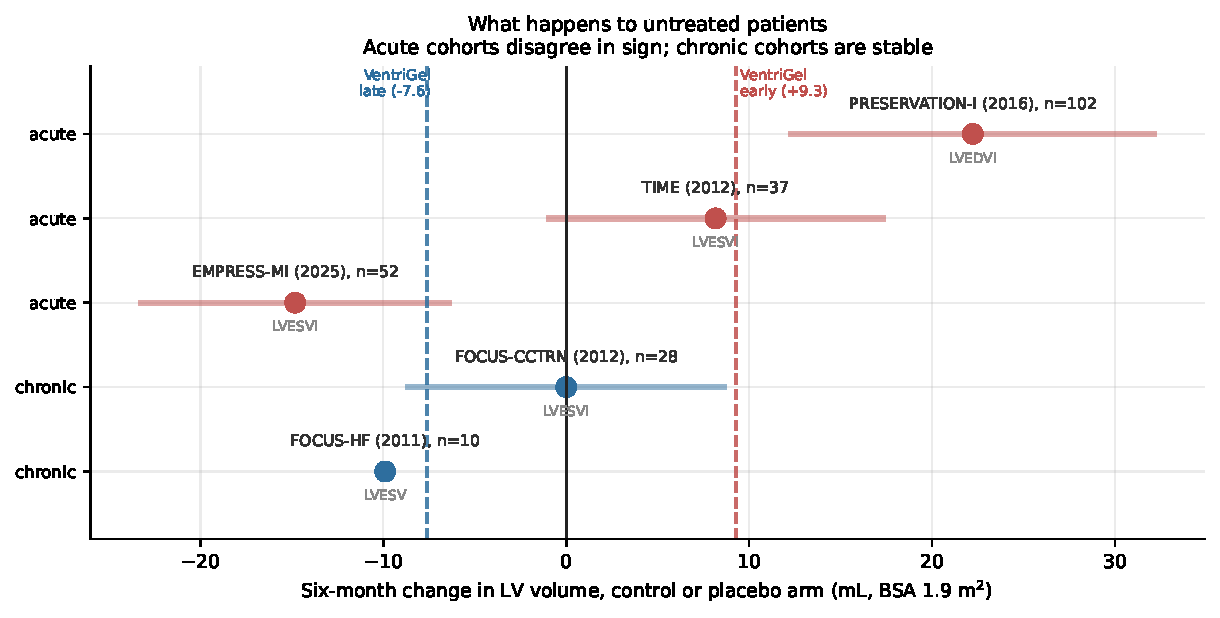
\includegraphics[width=\columnwidth]{../results/figures/fig3_literature_anchors.pdf}
\caption{Control and placebo arms of five randomized trials, converted to absolute volumes. Acute
cohorts disagree in sign; chronic cohorts are stable. Dashed lines mark VentriGel's own observed
stratum changes.}
\label{fig:anchors}
\end{figure}

Figure~\ref{fig:anchors} replaces the single-arm design's missing comparator with measurements. The
result is more interesting than a single number.

For \emph{acute} patients the anchors disagree in sign. TIME reported placebo-arm end-systolic
volume index rising 4.3\,mL/m$^2$ and PRESERVATION-I reported saline-arm diastolic index rising
11.7\,mL/m$^2$, but EMPRESS-MI, enrolling 2022--2024 on contemporary guideline-directed therapy,
reported end-systolic index \emph{falling} 7.8\,mL/m$^2$ with ejection fraction rising 8.5 points.
Post-infarction natural history is era-dependent: modern revascularization and medical therapy
produce functional recovery where older cohorts dilated. No single early-stratum control value is
defensible, so the range $-14.8$ to $+8.2$ mL is carried through every downstream result.

For \emph{chronic} patients the picture is stable. FOCUS-CCTRN --- the closest match to VentriGel's
late stratum on chronicity, the LVEF\,$\leq$\,45\% criterion and the transendocardial delivery route
--- observed a placebo-arm change of exactly zero. FOCUS-HF, with only ten control patients,
observed $-9.9$ mL and supplies a pessimistic bound.

Notably, TIME's $+8.2$ mL is close to VentriGel's early-stratum $+9.3$ mL. Under that anchor the
early stratum's apparent deterioration is largely natural history rather than treatment harm.

\subsection{The pooled effect is a cancellation}

\begin{figure*}[t]
\centering
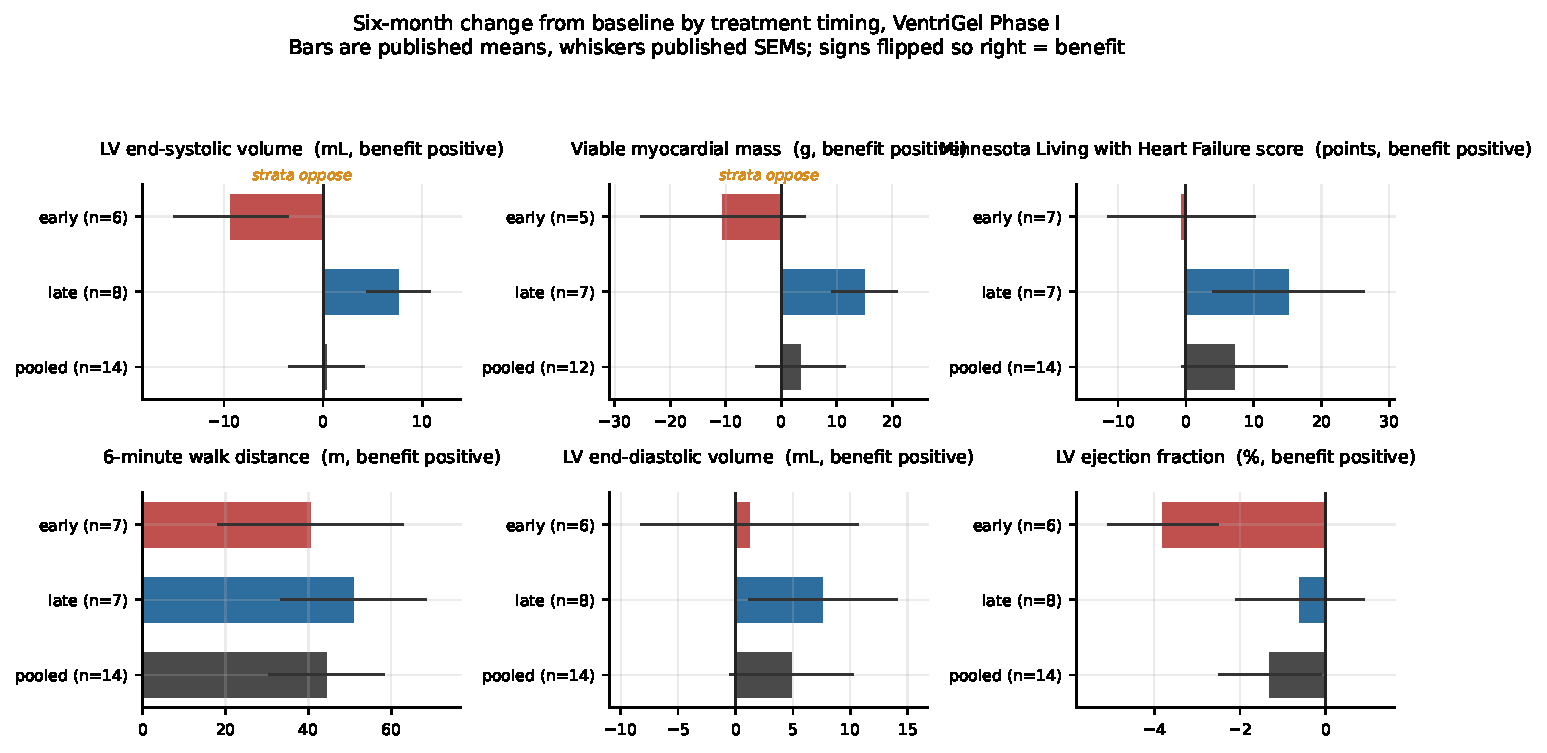
\includegraphics[width=\textwidth]{../results/figures/fig1_subgroup_cancellation.pdf}
\caption{Six-month change from baseline by treatment timing. Bars are published means, whiskers
published standard errors, signs flipped so right is benefit. For end-systolic volume and viable
mass the strata move in opposite directions, so the pooled bar is the residue of two offsetting
effects rather than a small common one.}
\label{fig:cancel}
\end{figure*}

Figure~\ref{fig:cancel} shows why the pooled numbers mislead. For end-systolic volume the early
stratum worsened by 9.3 mL while the late stratum improved by 7.6 mL, giving a pooled $-0.35$ mL
that is not a weak effect but two comparable effects of opposite sign. Viable mass shows the same
geometry more dramatically ($-10.5$\,g against $+15.0$\,g) but, as Section~3.2 established, its
interaction is not distinguishable from noise; it is reported as supporting rather than primary.

\subsection{Sample size under enrichment}

\begin{table}[t]
\centering
\small
\caption{Total randomized patients, $\alpha=0.05$, 80\% power, 10\% dropout, $\pi=0.53$, 25\%
discount. Volume endpoints use anchored controls (early $+8.2$, late $0.0$ mL); others assume no
drift and are correspondingly optimistic. Effects are signed so positive is benefit.}
\label{tab:n}
\begin{tabular}{lrrrr}
\toprule
Endpoint & $\Delta$ unsel. & $N$ unsel. & $\Delta$ enr. & $N$ enr. \\
\midrule
LVESV (mL)         & $2.64$  & 1{,}046 & $5.70$  & 92 \\
Viable mass (g)    & $2.32$  & 5{,}230 & $11.25$ & 70 \\
MLWHFQ (pts)       & $5.79$  & 958     & $11.32$ & 242 \\
LVEDV (mL)         & $6.32$  & 390     & $5.70$  & 366 \\
6-min walk (m)     & $34.53$ & 86      & $38.17$ & 56 \\
Ejection fr.\ (\%) & $-1.57$ & \emph{none} & $-0.45$ & \emph{none} \\
\bottomrule
\end{tabular}
\end{table}

\begin{figure*}[t]
\centering
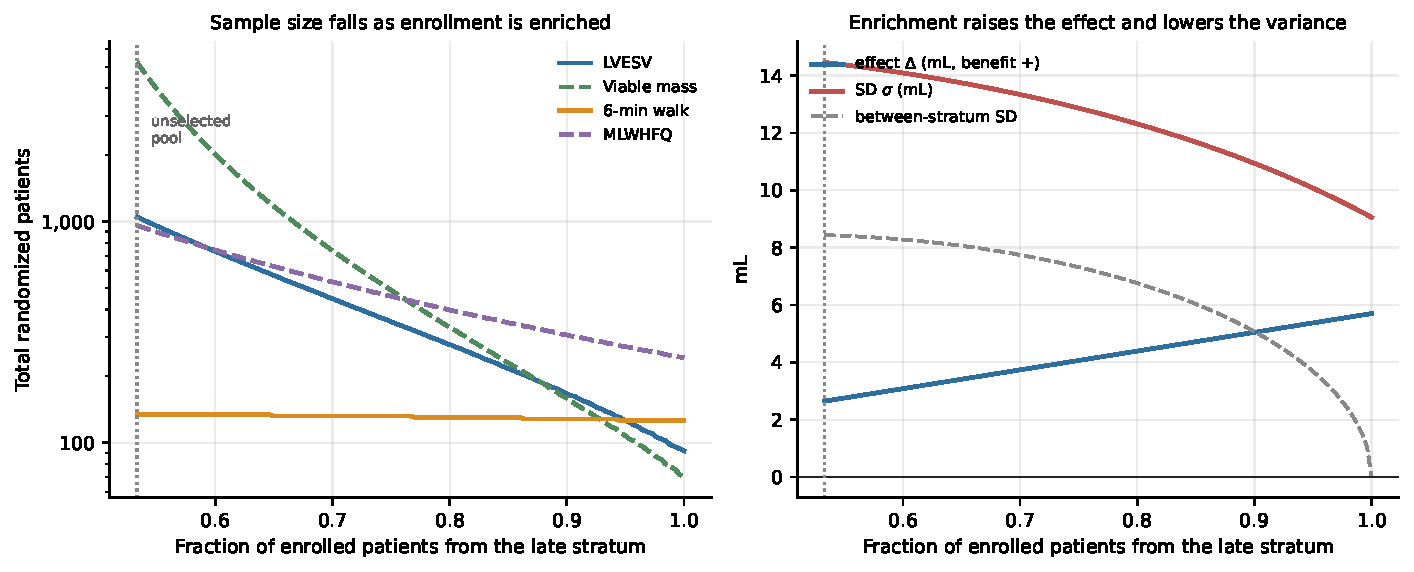
\includegraphics[width=\textwidth]{../results/figures/fig4_enrichment_curves.pdf}
\caption{Left: required sample size against enrichment level. Right: the mechanism for end-systolic
volume --- enrichment raises the effect and lowers the standard deviation simultaneously, because
the between-stratum variance component is eliminated.}
\label{fig:curves}
\end{figure*}

Table~\ref{tab:n} and Figure~\ref{fig:curves} give the design consequences. Under anchored controls
an unselected end-systolic volume trial requires 1{,}046 patients against 92 enriched, an
elevenfold difference. Moving from $e=\pi$ to $e=1$ raises the effect from 2.64 to 5.70 mL while
lowering the standard deviation from 14.3 to 9.1 mL, and the two gains compound in
$\sigma^2/\Delta^2$.

Enrichment is not uniformly useful, and the pattern is the paper's most transferable finding. For
six-minute walk distance both strata improve, so enrichment buys only about 1.5-fold and an
unselected trial of 86 patients is already feasible. For ejection fraction enrichment is
counterproductive: the pooled signal exists only because the early stratum deteriorated, so
restricting enrollment removes it. That signal is a possible safety observation rather than an
efficacy one, which makes its removal a governance question and not merely a statistical
inconvenience. The governing quantity is the sign of the effect in the stratum being excluded.

\subsection{Power is not probability of success}

\begin{figure*}[t]
\centering
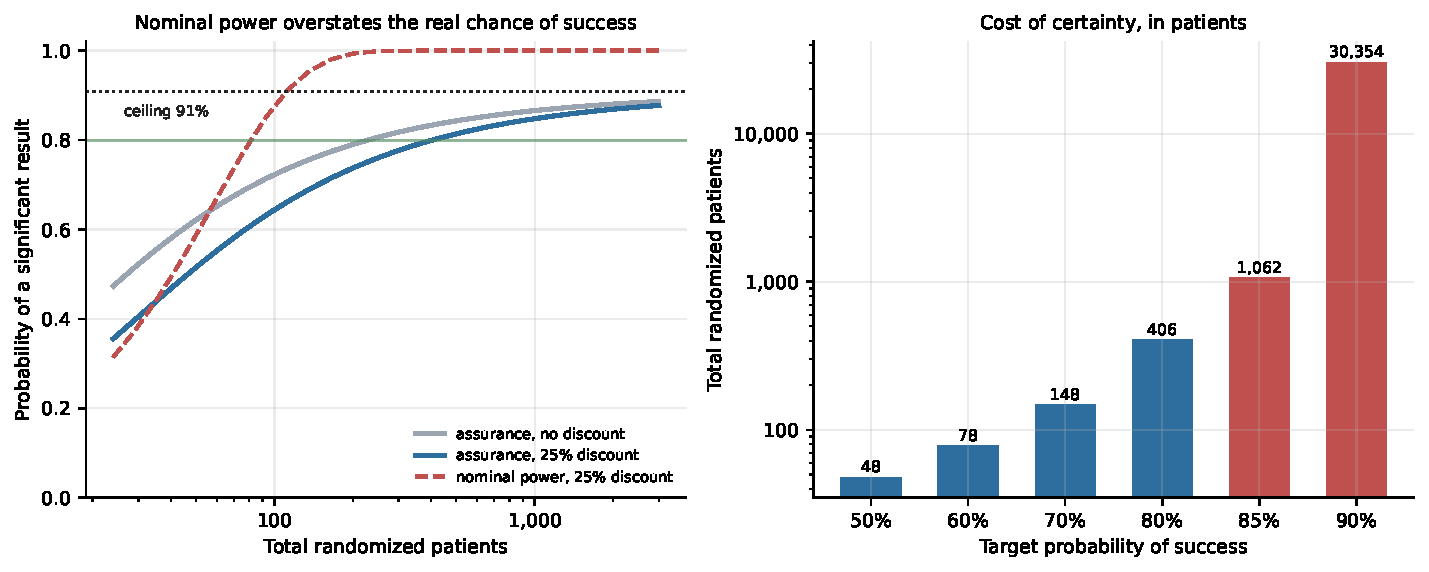
\includegraphics[width=\textwidth]{../results/figures/fig5_assurance.pdf}
\caption{Left: nominal power against assurance for the enriched design. Right: enrollment required
for a target probability of success. Assurance is bounded above by 97.5\%, the share of plausible
effects that point toward benefit at all.}
\label{fig:assurance}
\end{figure*}

Figure~\ref{fig:assurance} contains the most consequential correction in the analysis. The 92-patient
design solved for 80\% power at the point estimate has an assurance of 67.7\%. Genuine 80\%
probability of success requires 174 patients; 85\% requires 252 and 90\% requires 442.

Assurance also plateaus. No sample size exceeds 97.5\%, because that is the share of plausible
effects pointing toward benefit at all, and enrollment cannot fix an effect that is not there. That
ceiling is the honest expression of what a fifteen-patient single-arm trial can promise.

\subsection{Which assumption the conclusion rests on}

\begin{figure}[t]
\centering
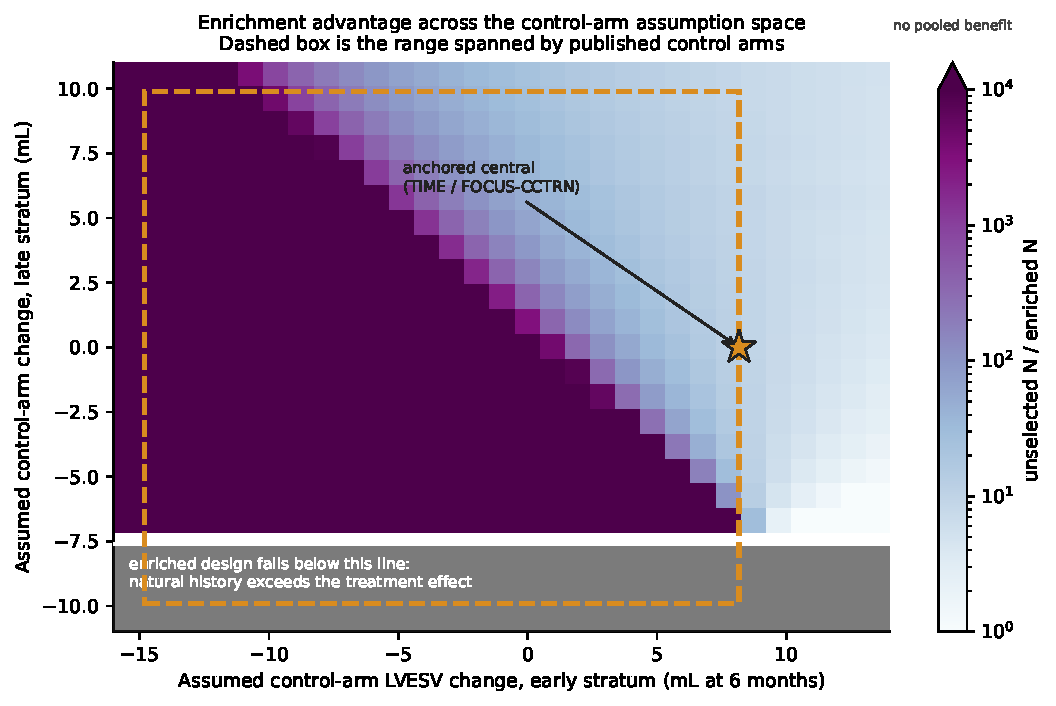
\includegraphics[width=\columnwidth]{../results/figures/fig6_control_drift.pdf}
\caption{Enrichment advantage across the control-arm assumption space with a 25\% discount applied.
The dashed box spans the published anchors and the star marks the anchored central case. Below the
white line the enriched design fails outright, because assumed natural history exceeds the treatment
effect.}
\label{fig:drift}
\end{figure}

Figure~\ref{fig:drift} maps the full assumption space, and the structure is asymmetric in a way that
matters. The enriched design enrolls no early patients, so its own size is unaffected by the
early-stratum assumption; what that assumption changes is the unselected comparator, and therefore
the size of the claimed advantage. The enriched design depends entirely on the \emph{late} stratum
assumption.

Under FOCUS-CCTRN's zero the design stands at 92 patients. Under FOCUS-HF's $-9.9$ mL, VentriGel's
$-7.6$ mL is smaller than natural history, the effect vanishes, and no trial is worth running. One
number decides the project, and the two available estimates of it disagree.

Sweeping the winner's-curse discount across its full range from 0.40 to 1.00 leaves the enriched
trial between 52 and 312 patients. No single discount is defended; the range is the claim.

\subsection{Estimation uncertainty and feasibility}

\begin{figure}[t]
\centering
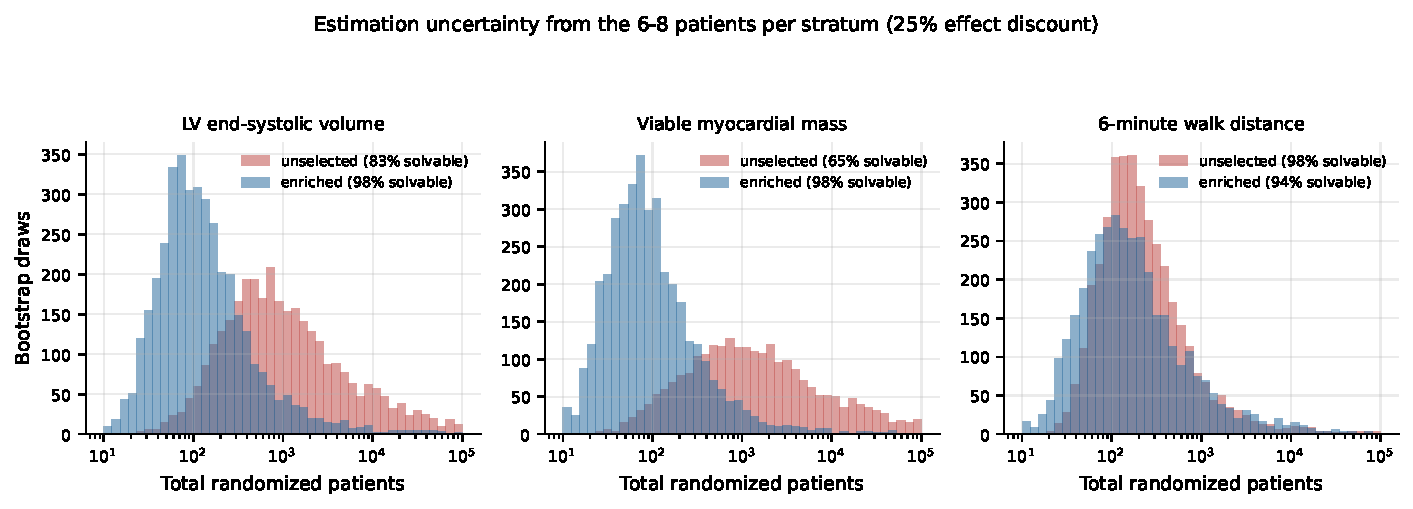
\includegraphics[width=\columnwidth]{../results/figures/fig7_bootstrap.pdf}
\caption{Bootstrap distributions of required enrollment. Intervals are wide because six to eight
patients per stratum cannot pin a sample size precisely.}
\label{fig:boot}
\end{figure}

\begin{figure}[t]
\centering
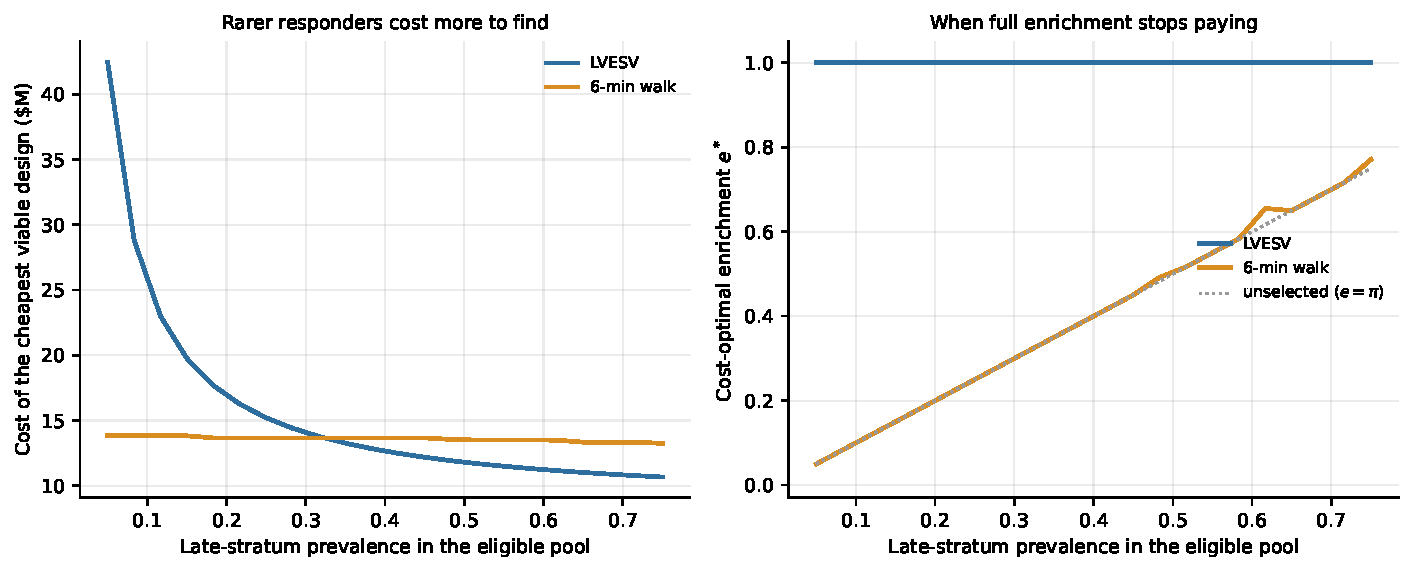
\includegraphics[width=\columnwidth]{../results/figures/fig8_economics.pdf}
\caption{Cost of the cheapest viable design as responders become scarcer, and the enrichment level
at which full enrichment stops paying.}
\label{fig:econ}
\end{figure}

\begin{figure}[t]
\centering
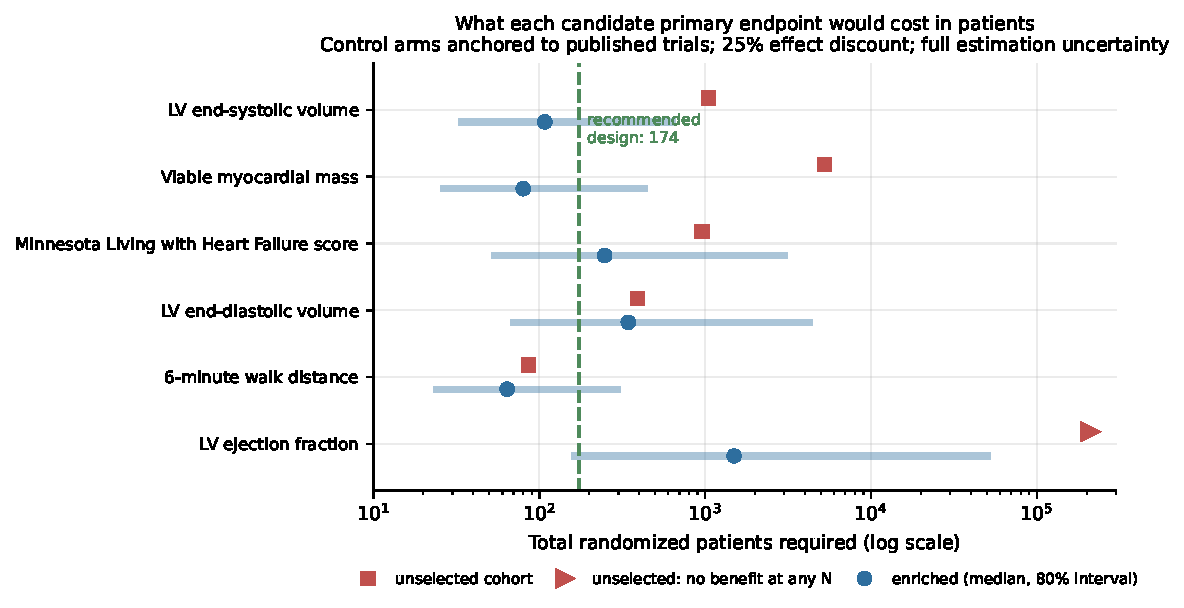
\includegraphics[width=\columnwidth]{../results/figures/fig9_design_summary.pdf}
\caption{Required enrollment per candidate primary endpoint, with the recommended 80\%-assurance
design marked.}
\label{fig:summary}
\end{figure}

Figures~\ref{fig:boot} and~\ref{fig:summary} report estimation uncertainty. The enriched end-systolic
volume design has a bootstrap median of 108 with an 80\% interval of 34 to 635 and 98\% of draws
favouring treatment. Reporting 92 without that interval would overstate the available precision.

Under the stated cost assumptions the 174-patient recommended design requires 326 screens, costs
approximately \$19.6M, and --- at the six sites that ran the Phase I --- would take 82 months to
enroll. Completing in 30 to 36 months instead requires 17 to 21 sites. This is a recruitment
finding rather than a statistical one, and it is the constraint a sponsor would encounter first.
Figure~\ref{fig:econ} shows the screening penalty binding as responders thin: for end-systolic
volume full enrichment always remains statistically optimal, because every early patient admitted
carries an effect of the wrong sign, whereas for six-minute walk distance a genuine interior optimum
appears.

\section{Discussion}

\subsection{What a sponsor should do}

If the reported pattern is real, a Phase II of VentriGel powered on left ventricular end-systolic
volume should restrict enrollment to patients more than twelve months post-infarction and plan for
approximately 174 randomized patients across 17 to 21 sites, accepting an 80\% probability of
success and understanding that the plausible range extends well beyond 600. An unselected trial on
the same endpoint should not be run, because the pooled estimate the Phase I supports is
indistinguishable from zero.

Before committing, a sponsor should measure the six-month end-systolic volume change in untreated
chronic post-infarction patients with LVEF\,$\leq$\,45\%. That single quantity is the horizontal axis
of Figure~\ref{fig:drift}; it separates a viable programme from an unviable one, and it is
obtainable from existing observational cohorts with serial cardiac magnetic resonance without any
new trial.

\subsection{The transferable point}

Describing heterogeneity as ``dilution'' obscures the decision that matters. Dilution implies a
recoverable effect and a larger trial; cancellation implies no recoverable effect and no viable
trial. Distinguishing them requires subgroup-level estimates, which are frequently published, and
requires reading a small pooled mean as a question rather than an answer. It also requires testing
the interaction, which is reported far less often than the within-subgroup comparisons that invite
the wrong conclusion.

\subsection{Limitations}

The interaction that motivates the entire analysis does not survive multiplicity correction. It is
one nominally significant result among nine, from a post hoc subgroup, in a fifteen-patient
single-arm trial. The strata contribute six and eight patients for the imaging endpoints. The
discount and bootstrap address the resulting fragility but cannot eliminate it, and the analysis
should be read as conditional throughout.

The single-arm design is the dominant structural limitation. External anchoring improves on an
arbitrary sweep but substitutes a different population for the missing control arm, and the acute
anchors disagree in sign. Body surface area was not reported and had to be assumed for unit
conversion. Cardiac magnetic resonance follow-up was incomplete, so stratum $n$ varies by endpoint.
The prevalence of late-stratum patients in a real eligible pool is unknown; the trial enrolled the
strata deliberately balanced, so its 8/15 split estimates its own design rather than the population.
Unit costs are planning assumptions.

Finally, statistical detectability is not clinical importance. A 7.6 mL reduction on the late
stratum's 142.3 mL baseline is a 5.3\% change, modest against the reverse-remodeling thresholds usually considered
clinically meaningful. A trial powered for the effect estimated here would establish that the effect
exists, not that it is worth having; powering for a clinically motivated target would increase every
figure in Table~\ref{tab:n}.

\section{Reproducibility}

All results are generated by \texttt{python run\_analysis.py} and \texttt{python make\_figures.py}
in about a minute, with no arguments and no downloaded data. Published values are transcribed in
\texttt{ventrigel/trial\_data.py} with the source table recorded for each, and external anchors in
\texttt{ventrigel/literature.py} with full citations. The validation of Section~3.1 and the
inference of Section~3.2 run on every execution, so a transcription error surfaces as a failed check
rather than a silently wrong result. A test suite covers the power mathematics against textbook
reference values.

\begin{thebibliography}{9}
\footnotesize

\bibitem{traverse2019}
Traverse JH, Henry TD, Dib N, Patel AN, Pepine C, Schaer GL, DeQuach JA, Kinsey AM, Chamberlin P,
Christman KL. First-in-man study of a cardiac extracellular matrix hydrogel in early and late
myocardial infarction patients. \textit{JACC Basic Transl Sci}. 2019;4(6):659--669.

\bibitem{singelyn2009}
Singelyn JM, DeQuach JA, Seif-Naraghi SB, Littlefield RB, Schup-Magoffin PJ, Christman KL. Naturally
derived myocardial matrix as an injectable scaffold for cardiac tissue engineering.
\textit{Biomaterials}. 2009;30(29):5409--5416.

\bibitem{seifnaraghi2013}
Seif-Naraghi SB, Singelyn JM, Salvatore MA, et al. Safety and efficacy of an injectable extracellular
matrix hydrogel for treating myocardial infarction. \textit{Sci Transl Med}. 2013;5(173):173ra25.

\bibitem{traverse2012}
Traverse JH, Henry TD, Pepine CJ, et al. Effect of the use and timing of bone marrow mononuclear cell
delivery on left ventricular function after acute myocardial infarction: the TIME randomized trial.
\textit{JAMA}. 2012;308(22):2380--2389.

\bibitem{rao2016}
Rao SV, Zeymer U, Douglas PS, et al. Bioabsorbable intracoronary matrix for prevention of ventricular
remodeling after myocardial infarction. \textit{J Am Coll Cardiol}. 2016;68(7):715--723.

\bibitem{carberry2025}
Carberry J, Petrie MC, Lee MMY, et al. Empagliflozin to prevent worsening of left ventricular volumes
and systolic function after myocardial infarction (EMPRESS-MI). \textit{Eur J Heart Fail}.
2025;27(3):566--576.

\bibitem{perin2012}
Perin EC, Willerson JT, Pepine CJ, et al. Effect of transendocardial delivery of autologous bone
marrow mononuclear cells on functional capacity, left ventricular function, and perfusion in chronic
heart failure: the FOCUS-CCTRN trial. \textit{JAMA}. 2012;307(16):1717--1726.

\bibitem{perin2011}
Perin EC, Silva GV, Henry TD, et al. A randomized study of transendocardial injection of autologous
bone marrow mononuclear cells and cell function analysis in ischemic heart failure (FOCUS-HF).
\textit{Am Heart J}. 2011;161(6):1078--1087.

\bibitem{fda2019}
U.S. Food and Drug Administration. \textit{Enrichment Strategies for Clinical Trials to Support
Determination of Effectiveness of Human Drugs and Biological Products: Guidance for Industry}.
March 2019.

\bibitem{temple2010}
Temple R. Enrichment of clinical study populations. \textit{Clin Pharmacol Ther}.
2010;88(6):774--778.

\bibitem{wang2007}
Wang R, Lagakos SW, Ware JH, Hunter DJ, Drazen JM. Statistics in medicine --- reporting of subgroup
analyses in clinical trials. \textit{N Engl J Med}. 2007;357(21):2189--2194.

\bibitem{sun2010}
Sun X, Briel M, Walter SD, Guyatt GH. Is a subgroup effect believable? Updating criteria to evaluate
the credibility of subgroup analyses. \textit{BMJ}. 2010;340:c117.

\bibitem{benjamini1995}
Benjamini Y, Hochberg Y. Controlling the false discovery rate: a practical and powerful approach to
multiple testing. \textit{J R Stat Soc Series B}. 1995;57(1):289--300.

\bibitem{ohagan2005}
O'Hagan A, Stevens JW, Campbell MJ. Assurance in clinical trial design. \textit{Pharm Stat}.
2005;4(3):187--201.

\bibitem{senn2004}
Senn S. Individual response to treatment: is it a valid assumption? \textit{BMJ}.
2004;329(7472):966--968.

\bibitem{wong2019}
Wong CH, Siah KW, Lo AW. Estimation of clinical trial success rates and related parameters.
\textit{Biostatistics}. 2019;20(2):273--286.

\bibitem{moore2018}
Moore TJ, Zhang H, Anderson G, Alexander GC. Estimated costs of pivotal trials for novel therapeutic
agents approved by the US Food and Drug Administration, 2015--2016. \textit{JAMA Intern Med}.
2018;178(11):1451--1457.

\end{thebibliography}

\end{document}
